\documentclass{article}
\usepackage[utf8]{inputenc}
\usepackage[English]{babel}


\usepackage{graphicx}
\usepackage[colorlinks=true, allcolors=blue]{hyperref}
\usepackage{caption,subcaption}
\captionsetup[subfigure]{labelformat=empty}

\title{Secure Shell Project}
\author{}
\date{January 2023}

\begin{document}

\maketitle

\section{Introduction}


\section{What is SSH?}
SSH (Secure Shell) is used for managing networks, operating systems, and configurations. It is also inside many file transfer tools and configuration management tools. Every major corporation uses it, in every data center.

\subsection{The SSH protocol}
The SSH protocol uses encryption to secure the connection between a client and a server. All user authentication, commands, output, and file transfers are encrypted to protect against attacks in the network. 

\begin{figure}[!h]
    \centering
    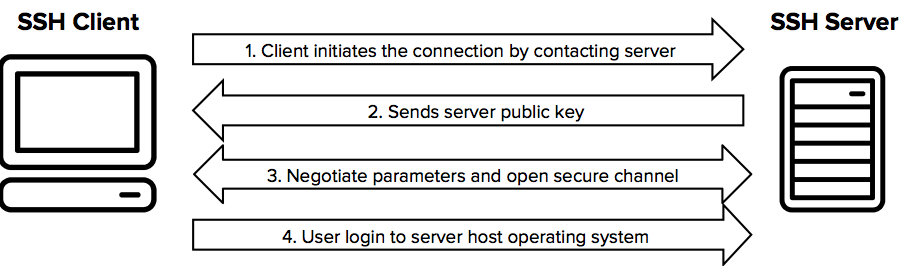
\includegraphics[width=1 \textwidth]{ssh protocol.png}
    \caption{SSH Protocol}
    \subcaption{source: ssh.com/academy}
\end{figure}


\subsection{Automate with SSH keys, but manage them}
SSH keys can be used to automate access to servers. They are commonly used in scripts, backup systems, configuration management tools, and by developers and sysadmins. They also provide single sign-on, allowing the user to move between his/her accounts without having to type a password every time. This works even across organizational boundaries, and is highly convenient.

However, unmanaged SSH keys can become a major risk in larger organizations.




\subsection{History of the SSH protocol}
The Secure Shell protocol was originally developed by Tatu Ylonen in 1995 in response to a hacking incident in the Finnish university network. A password sniffer had been installed on a server connected directly to the backbone, and when it was discovered, it had thousands of usernames and passwords in its database, including several from Ylonen's company.

That incident triggered Ylonen to study cryptography and develop a solution he could use himself for remote login over the Internet safely. His friends proposed additional features, and three months later, in July 1995, Ylonen published the first version as open source. It became OpenSSH. Later he took the protocol for standardization at the IETF and designed the SSH File Transfer Protocol (SFTP). He founded SSH Communications Security Corp in December 1995 to provide commercial support for the protocol.

Ylonen still works on topics related to Secure Shell, particularly around key management, as well as broader cybersecurity topics.

\subsection{SSH keys are a critical access management problem}
SSH keys provide the same access as user names and passwords. Furthermore, they often grant access to privileged accounts on the operating system level, giving a command line. Yet, in many cases, SSH keys have been completely overlooked in identity and access management planning, implementation, and audits. Users have been able to create and install keys without oversight and controls. This has led to violations of corporate access policies and dangerous backdoors.

Over the last few years, it has turned out that most large organizations have massive numbers of SSH keys in their environment. These keys are like passwords. They grant access to resources - production servers, databases, routers, firewalls, disaster recovery systems, financial data, payment systems, intellectual property, and patient information.

Information security starts from controlling who is given access to systems and data. If there is no control over access, there is no security, no confidentiality, no integrity, and no guarantees of continued operation.


\subsection{Insight from real customer cases}
We have worked with many companies, including several global top-10 banks, leading retailers, and other large Fortune 500 companies. Based on our findings, most organizations:

Have extremely large numbers of SSH keys - even several million - and their use is grossly underestimated

Have no provisioning and termination processes in place for key based access

Have no records of who provisioned each key and for what purpose

Allow their system administrators to self-provision permanent key-based access - without policies, processes, or oversight.

In the case of one representative customer, we went through a quarter of their IT environment as part of a major SSH key management project. They had five million daily logins using SSH, most of them using SSH keys for automation. We analyzed 500 business applications, 15000 servers, and found three million SSH keys that granted access to live production servers.

\newpage

\section{Key Exchange}
SSH keys are authentication credentials. Functionally SSH keys resemble passwords. They grant access and control who can access what. 
SSH key exchange (sometimes called KEX) is used by the client and server to exchange information in public that leads to a secret shared by the client and server that an observer can not discover or derive from public information.

\begin{figure}[!h]
    \centering
    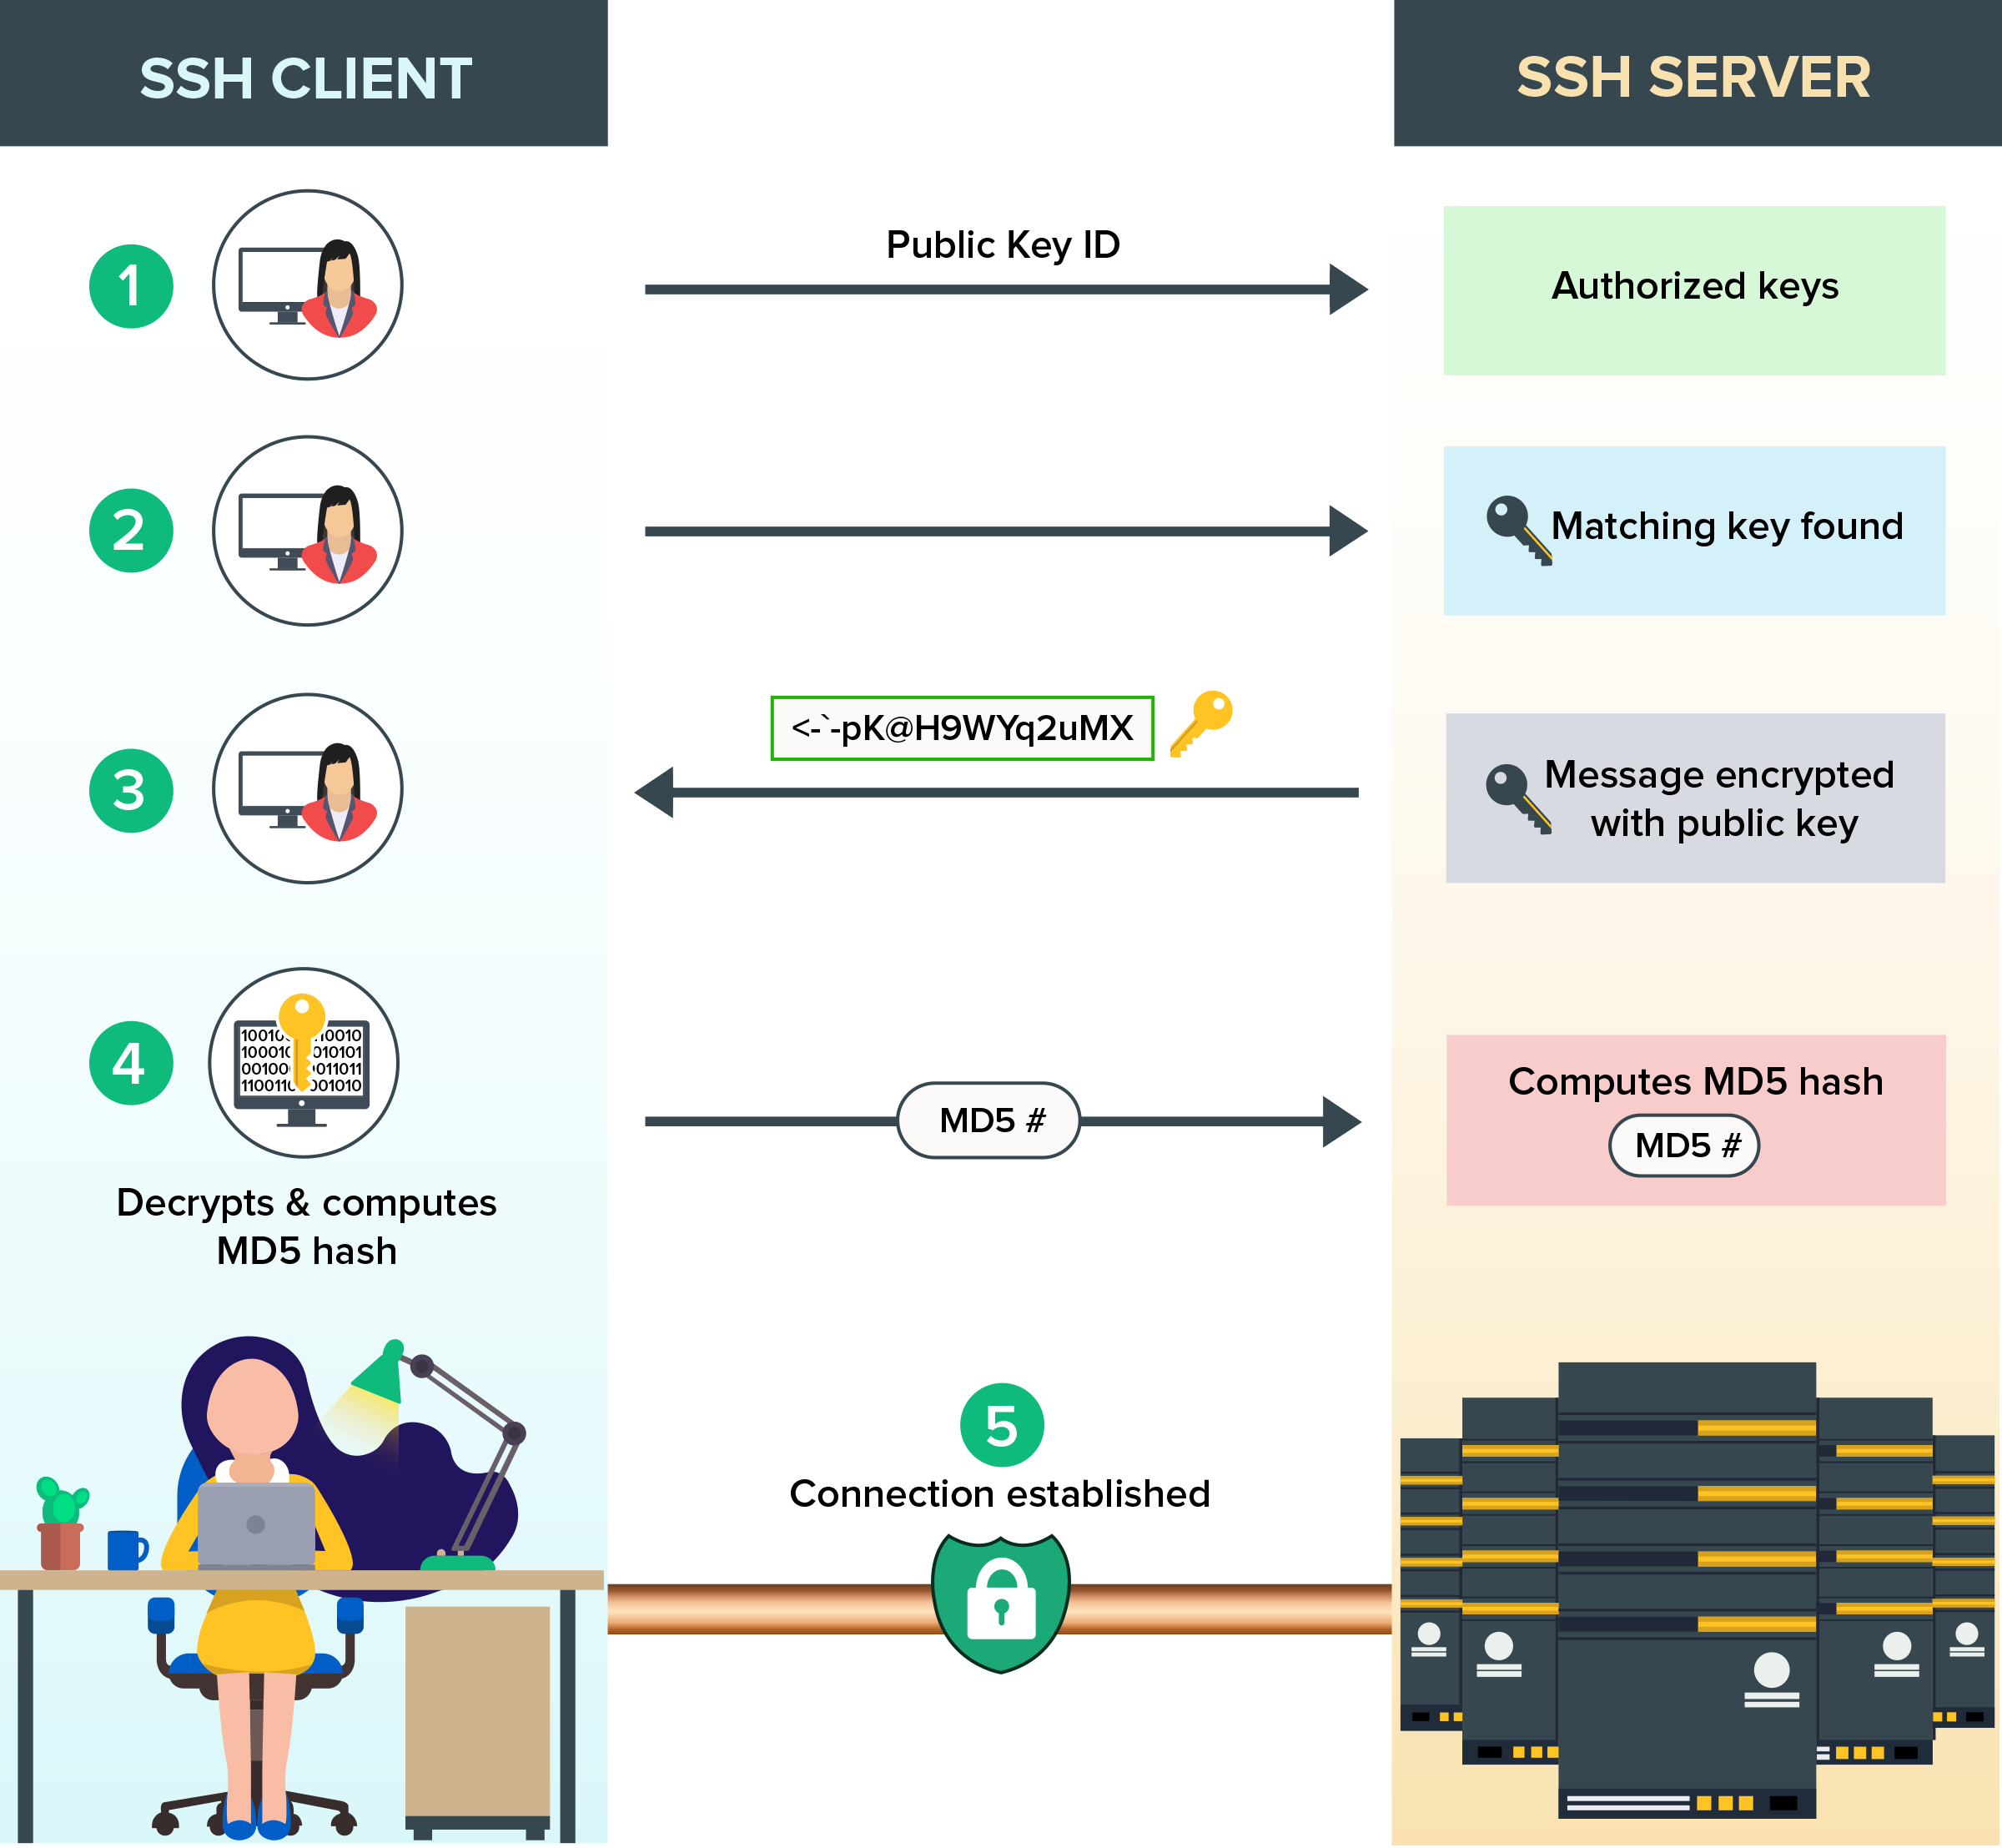
\includegraphics[width=1 \textwidth]{keyExchange.png}
    \caption{Key Exchange}
    \subcaption{source: manageengine.com}
\end{figure}


\subsection{The risk of unmanaged SSH keys}
Unmanaged access exposes organizations to significant risks that could in the worst case bring down critical information systems for months. Unmanaged keys risk systemic failure of critical infrastructure, especially in a cyberwarefare scenarios.

\subsubsection{Stolen and misused keys}
There are far more SSH keys in circulation than anyone seems to believe. In one financial sector customer case we encountered 3 million keys (750,000 distinct keypairs) from 15,000 servers. In another case there were 4.5 million authorized keys from 100,000 servers. Typical numbers for Fortune 500 companies range from hundreds of thousands to millions - many times more than they have employees or system administrators with command line operating access.

With so many unmanaged keys the likelihood of keys being misused, stolen, or used as part of an attack is high. One single key can be enough to gain undetected access to critical systems and data.

\subsubsection{The impact of compromise is very high}
We have found that in several customer cases about 10percent of the discovered keys grant root access. An attacker getting root means they can do anything on the server - including inject fraudulent data, subvert encryption software, install persistent malware, or outright destroy the system. Confidentiality, integrity, and continuity of operations are all compromised. Even if the key gives non-root access, local privilege escalation vulnerabilities can often result in the attacker gaining root access.

There is substantial risk that SSH keys can be used to spread an attack to a majority of all production servers in the organization. This could cause billions of dollars of damage to shareholders. Many companies use SSH keys to push data to disaster recovery sites and backup systems, exposing them to attacks as well.

\subsection{Our solutions to SSH key management}
The role of SSH, the company, in SSH key management projects is typically to provide best-of-breed software, best subject matter expertise, and help to structure and manage the project and define SSH-related policies. We typically provide 1-2 subject matter experts for larger projects to work with the customer's engineers or outsourcing partners.

\subsubsection{Universal SSH Key Manager®}
Universal SSH Key Manager is our flagship product for managing SSH keys. It has been used by numerous large and mid-sized organizations for solving their key management problems. It handles the entire lifecycle for key-based access, and integrates to leading identity and access management systems, privileged access and privilege elevation systems, as well as SIEM (Security Information and Event Management) and configuration management.

Together with consulting services, Universal SSH Key Manager makes it easy for customers to solve their key management issues. We also can run the whole project for you, working with your application teams and identity & access management, cryptography, security engineering, operations, and/or IT transformation groups as needed, globally. We've run SSH key management projects in the US, UK, Germany, and Singapore, among others.

\bibliographystyle{alpha}
\bibliography{sample}

\href{https://www.ssh.com/academy/ssh} {SSH Academy}

\href{https://goteleport.com/blog/ssh-handshake-explained/} {SSH Handshake Explained}


\end{document}
